\section{Data Description}

\subsection{Prices, Exchanges, and Coin charactertistics}


%\begin{figure}[h]
%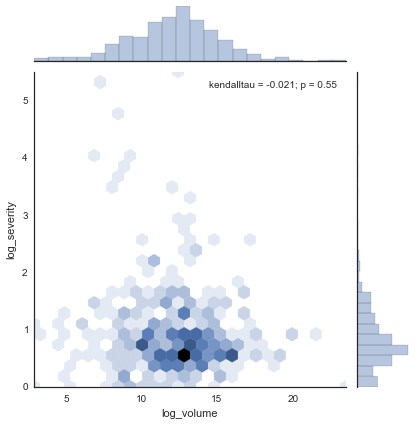
\includegraphics[width=\columnwidth]{severtiy_volume}
%\end{figure}

Our main outcome measures are the severity of drop in the value of a unit of the asset, and the magnitude in USD of the transactions in them.
To obtain data for them we scrape three market aggregators 

We operationalize the intensity of a bubble as the proportion of a 1 dollar that would be lost buying at the maximum price and selling after that proportionally to the volume of the market till the present, we call this severity.
We define the volume as the sum of the contemporaneous dollar (todo check) volume of trade.

As a secondary outcome measure we consider the number of exchanges that list the coin.


\subsection{Forum Discussions}

In order to study the effect of communication network around cryptocoins on
price variations, we collected all the posts from the most popular cryptocurrency
online community, bitcointalk.  Our data consisted of all the posts that were
made between January 2010 and July 2015 on the most active crypto-related forums:
\begin{enumerate}[topsep=0pt,itemsep=-0.5ex,partopsep=1ex,parsep=1ex]
  \item \textbf{Bitcoin Discussion:} This is the oldest forum on the website which mainly focuses
    on issues only related to Bitcoin. Interestingly, Satoshi Nakamoto, the alleged
    creator of Bitcoin made the first post on this forum in January 2010 and
    was active until January 2011. The presence of Satoshi in the data set enables us
    to study the position of various actors in the online community relative to Satoshi
    and its relation with the success or failure of cryptocoins they advocate or reject.
  \item \textbf{Altcoin Discussion:} This is the most active forum in the community
    with more than 730,000 posts as of July 2015, and dating back to June 2011.
    The discussions in this forum mainly evolve around alternative currencies
    other than Bitcoin. Users often discuss the merits or flaws of various
    altcoins or simply exchange technical information.
  \item \textbf{Announcement (Altcoin):} Community announcements such as development of 
    exchange client or addition of new features are made here. This is an important forum
    in our study as the creation of new altcoins are announced here. Whenever a new
    altcoin is announced to the community, the announcement is tagged with string ANN.
    This enables us to detect announcement of new coins into the market and identify
    the users who introduced them for the first time.
  \item \textbf{Mining (Altcoin):} Technical issues pertaining to mining (i.e. validating transactions)
    altcoins are discussed here.
  \item \textbf{Marketplace (Altcoin):} This forum contains the discussions on a wide-range of 
    market-related issues, such as price or volume trends, possible pump and dump schemes
    and exchange tips.
\end{enumerate}

TODO:Do we want any other descriptive stats on the forum other than those mentioned here? 

Each forum consists of many subjects or threads initiated by different users.
Each thread contains several posts or replies, with an average of 10 posts per
thread.  The reply structure within each thread constitutes the basis of our
forum network, discussed below.  Each post has several fields which contain
valuable information in our context.
\begin{enumerate}[topsep=0pt,itemsep=-0.5ex,partopsep=1ex,parsep=1ex]
  \item \textbf{Subject:} Usually, the initiator of the thread chooses subject and all the
    following posts inherit the same subject.
  \item \textbf{Content:} The actual text of the post.
  \item \textbf{Position in the thread}: The later posts in the thread might not be as important
    as earlier posts and could be about issues other than the original topic of the thread.
  \item \textbf{Author}
  \item \textbf{Date}
\end{enumerate}
The community had only 10000 unique users until early 2013, however it grew considerably faster after 2013 and reached about 70000 by early 2015.
Nevertheless, there are only 10000 active users within any 30 day period on average.

\section{Forum Interaction Network}

Given the forum discussion data at the level of individual posts, we  construct a network capturing the discussion patterns among users. The structural properties of this network form the basis of our analysis on a per-coin basis. In this network, nodes are the forum users and \textit{directed edges} point from posters within each thread to thread-initiators. The omission of edges based on simple co-appearance within a thread leads to a sparser network which isolates the communication patterns around ``dialogue-shapers''. The edges in the discussion network are weighted by the number of times a poster replies to a thread-initiator in different threads (i.e. multiple replies by the same user within the same thread count only as once).
% Is this too big of a statement?
In this context, edge weights capture the level of engagement thread initiators receive from the community and the amount of information a poster receives from thread initiators. Furthermore, our network construction method uses all the interactions since the inception of bitcointalk in creating new edges or updating their weights. The unlimited retention of any such (replier to thread initiator) interaction captures relevant information on seniority and community influence which are obtained through long-term and persistent presence in the forums. 

Prior to construction of the network, we merged posts from all forums into a
single large forum since the community base of all five forums mentioned
above is made of the same users and we are mostly concerned about influence and
aggregate information flow among users, rather than the exact topic of the discussion.
The network construction involves replaying all the posts over time sorted by their date and updating the
discussion network accordingly. Whenever a new altcoin is introduced
in the forum for the first time, the user who introduced it and a snapshot of the network is taken. 
We analyze the discussion network only up to the first time each coin is introduced to the community, in order to avoid any possible confounding between a coin's price movement and the extra attention it receives in the community due the same price changes. Our method uses the position of the first introducer in the network snapshot and the general structure of her neighborhood for extracting various network measures corresponding to that coin. Our final analysis examines these per-coin measures for evaluating the performance of each coin.



%TODO Do we use the date of the ANN or the date of the first trade?!?! NIKETE & EAMAN.
% E: Both of them are in the file, depends which one you are using. 
%The identification of true introductions of new altcoins is a difficult process prone to many false-positives. 
The  majority of such introductions are made in the \textit{Announcement} forum and are preceded with the ``ANN'' tag. We look for the first mention of both the coin symbol \textbf{and} its descriptive name in the subject of a thread which contains the announcement tag. The first mentions of either the coin symbol \textbf{or} the its name are used fall-back in case the more restrictive \textbf{and} requirement did not detect the coin. 
Using this method, we were able to detect the first introduction of 554 altcoins out of 679.
The forum user who initiated such a thread is assigned as the introducer of the coin to the community.

TODO: add validation results table wrt mapofcoins data here
